\Chapter{A virtuális kollaborációs tér}

% A fejezet gyakorlatilag a kliens kialakításáról szól.

% Maga a menü, beállítások és egyéb felületi elemek is lehetnek 3D-sek.

A dolgozat elsődleges célja, hogy egy AR/VR alapú kollaborációs teret hozzon létre.
A fejezet ennek a megjelenítési módjával és a virtuális térben való interakciónak a leírásával foglalkozik.

\Section{Megjelenítési mód}

A megjelenítési mód OpenGL alapú.
A következő szakaszokban ennek a Python nyelvű implementációja kerül részletezésre.

\SubSection{OpenGL, PyOpenGL}

Az OpenGL egy grafikus nyelv, amely függvénykönyvtár formájában rendelkezésre álló implementációjával 2D-s és 3D-s alakzatokat tudunk megjeleníteni. Nagyon elterjedt, elérhető és támogatott a fő operációs rendszereken (Linux, macOS, Windows), valamint számos programozási nyelvvel kompatibilis \cite{madsen2016opengl}.

Az OpenGL pythonnal használható verziója a cross-platform, nyíltforráskodú \textit{PyOpenGL}. A PyOpenGL támogatja a GL, GLU és GLUT könyvtárakat.
Továbbá lehetőség van a \textit{PyGame} függvénykönyvtár használatára OpenGL-s kódok megvalósításához.

A dolgozathoz tartozó program felhasználja mindhárom könyvtárat, és a modell betöltéshez a \textit{PyGame}-et is.

\SubSection{Modellek}

A program Wavefront OBJ formátumú modellekkel dolgozik, amelyekhez anyagjellemzőket leíró, \texttt{mtl} kiterjesztésű fájlokkal textúrát is rendelhetünk. 
\begin{itemize}
\item \texttt{obj}: A Wavefront Technologies által a Advanced Visualizer animációs csomagjukhoz kifejleszett obj fájlformátum egy geometria-definíciós formátum. 
Annak köszönhetően, hogy nyílt formátum, más 3D-s grafikus alkalmazások gyártói átvették.

Az obj egy egyszerű formátum ( akár ember által is olvasható), ami semmi mást nem add meg, mint a 3D geometriát, mint például a csúcsok helyzetét, az egyes textúra koordináta-csúcsok helyzetét, a csúcsok normálisát, az egyes sokszögeket csúcsok listájaként, textúra csúcsokat.

\item \texttt{mtl}: Az MTL fájl egy segédfájl, amely a modell anyagainak meghatározását tartalmazza, amelyekhez OBJ fájl hozzáférhet. Az OBJ fájlnak meg kell adnia az MTL fájl nevét. Az MTL fájl az anyagok definícióinak sorrendjét tartalmazza. Mindegyik definíció egy newmtl utasítással kezdődik, amely meghatározza az anyag nevét, majd azon sorok következnek, amelyek megadják az adott tulajdonságokot.
\end{itemize} 

A programok és demók elkészítéséhez a modelleket a modelleket ábrázoló képekhez társított forrásoldalakról töltöttem le.  

A program fő elemei az ágensek. 
A modell, amit felhasználtam erre a célra egy császárpingvin (\ref{fig:pingvin}. ábra). 
Minden ágenst ilyen modellel jelenít meg a program, csupán a színük változik, ami pedig a programkódban kerül megvalósításba.

\begin{figure}[htp]
    \centering
   	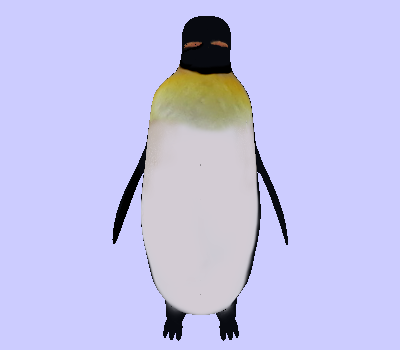
\includegraphics[scale=0.6]{images/pingvin.png}
	\caption{császárpingvin modell}
	\label{fig:pingvin}
\end{figure}

A program szinterének fő eleme a kastély modell, ahol maga a jelenet játszódik (\ref{fig:castle}. ábra).

\begin{figure}[htp]
    \centering
   	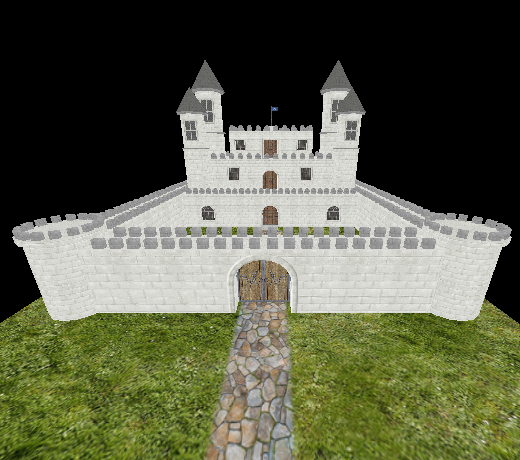
\includegraphics[scale=0.7]{images/castle.png}
	\caption{kastély modell}
	\label{fig:castle}
\end{figure}

Felhasználtam továbbá doboz modelleket, amiknek az elmozgatása a feladat (\ref{fig:box}. ábra). Ezen modellek színének manipulációja szintén a programban történik.

\begin{figure}[htp]
    \centering
   	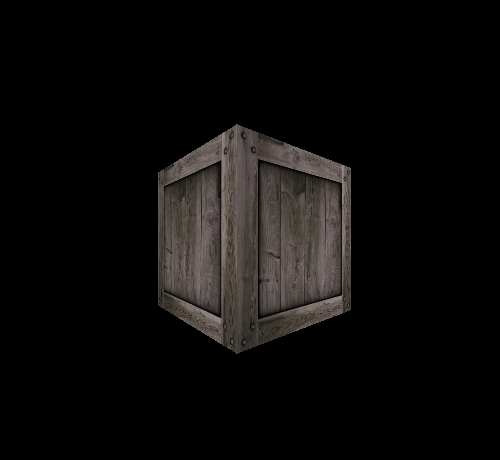
\includegraphics[scale=0.5]{images/box.png}
	\caption{doboz modell}
	\label{fig:box}
\end{figure}

\Section{Interaktív elemek}

A színtér interkatív elmei az ágensek és a dobozok. 
Az ágensek képesek fordulni, előrehaladni, ugorni. 
A dobozok pedig olyan irányú elmozdulásra, amerre tolják őket.

\SubSection{Animáció}

Ahhoz, hogy a program látványosabb legyen animációkra van szükség, így a modell nem csak elmozul például olyan irányba, amerre szeretnénk, hanem az animáció használata séta hatását kelti.

A modellek formátuma azonban nem támogatja az animációkat, ezért minden egyes mozdulatnak külön modell készült (a hozzátartozó mtl fájllal).

Az animációk elkészítéséhez elsőnek a modell úgynevezett vázára van szükség, azt kell elkészíteni, és azt lehet a továbbiakban animálni. 
 
Az elkészült animációk a következők: ugrás, séta és a dobozok tolásához a doboz megfogása és elengedése.

Az animáció elkészítéséhez a Blender nevű program lett felhasználva. 

Fontos, hogy minden egyes mozdulatot rajzolását úgy kell megvalósítani, hogy minden más modell és a kamera képből készült háttér is kirajzolódik.
 
\SubSection{Ütközésvizsgálat}

Az ágensek megfelelő térrészben tartása végett (tehát hogy ne tudják elhagyni a kastélyt, ne sétáljanak át egymáson, illetve más modelleken) szükség van ütközésvizsgálatra.
Ez azt jelenti, hogy figyeljük a modellek egymáshoz való helyzetét a térben, a távolságot közöttük, és ha túl közel kerülnek egymáshoz, akkor megakadályozzuk, hogy tovább haladjon a mozogni képes modell.
Ez azt jelenti, hogy  mozoghat  például az $y$ tengely mentén, ha az adott irányban nincs előtte akadály.
Ha mindkét művelettel akadályba ütközne, akkor nem haladhat az adott irányba.
 
Az első dolog, amit meghatároztam az az volt, hogy a $z$ tengelyen (ez jelenleg a fel és le írány a játékban) nem sülyedhet 0 alá az ágensek értéke, mert akkor a kastély modellbe és alá esne egy részük.

A következő lépésben a tér azon részét határoztam meg, ami a játékteret képezi (a kastély modell kertje), hogy a falakon ne tudjanak áthaladni a modellek, tehát tényleg ne legyenek képesek elhagyni a játék végéig.

Ez az $x$ és $y$ tengelyre jelent korlátozásokat.

A további lépés az ágensek poziciójának figyelése, hogy az ágensek egymáson ne tudjanak áthaladni. Ehhez minden pozició változás előtt meg kell vizsgálni, hogy az adott lépéssel nem kerülnek e a másik modell olyan közvetlen közelébe, ami már nem megengedett.

Mivel a pingvin modellek középpontja a modell közepébe esik, ezért egy bizonyos értéket mindig hozzá kell adni a számításkor (hogy a modell széleit figyeljük), hogy ne lógjanak egymásba semmilyen esetben sem. 

Az ágenseknél továbbá azt is figyelmbe kell venni, hogy a kódban át lettek méretezve, ezért a poziciójuk koordinátáit is a megfelelő arányban kell növelni/csökkenteni.

Ugyanez vonatkozik a doboz modellek való ütközésvizsgálatra, mindig lesz valamekkora plusz érték, ami a modell szélét hivatott jelenteni.

A programban ez egy olyan osztályban valósul meg, ami megkapja a tér modelljeit és azt a modellt, aminek figyelnie kell a pozicóját.
 
Minden lépés előtt ellenőrzi, hogy az adott lépéssel nem ütközne-e akadályba és csak akkor valósulhat meg a lépés, ha nincs akadály.

\Section{A kastély, mint játéktér}

A játék fő színhelye az előbb említett kastély modell, amiből nem lehet kijutni csak akkor, ha a karakterek teljesítik a rájuk kiszabott feladatot.

A kastély falain nem lehet átjutni és az ajtók sem használhatóak.

A feladat, amit el kell végeznie a karaktereknek az az, hogy a saját színűkhöz tartozó dobozokat kell a megfelelő helyre jutatniuk, ami jelen esetben a szökőkutak egyike. 

A szökőkutak közül egyszerre csak egy aktív (amelyik nincs takarva), csak azzal van lehetőség a dobozok eltűntetésére. Minden esteben az előforduló színek közül pontosan egy kerülhet az aktív szökőkútba (különben nem tűnik el, ha ugyanolyat próbálnak beletolni). Ha a megfelelő mennyiségű doboz eltűnik, akkor a másik kút lesz aktív.

Fontos, hogy minden játékos csak a saját színével megegyező színű dobozt képes mozgatni és csak azt szabad mozgatnia. Azonban csak az tilos, hogy eltolja, például hozzá érhet.

Ha nem a saját dobozát próbálja meg eltolni (például hamar végez és megpróbál segíteni a társának), akkor sem változik semmi, csupán egyhelyben jár.

Minden játékosnak a saját részét szabad csak megcsinália a kiszabott feladatból. 

A játékosoknak minden esetben együtt kell működniűk, mert csak akkor jutnak ki, ha minden doboz eltűnt. Ebben valósul meg a játék kooperatív jellege. 

\begin{figure}[htp]
    \centering
   	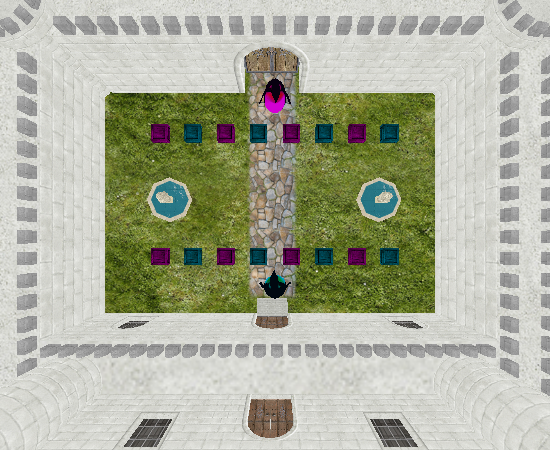
\includegraphics[scale=0.7]{images/game.png}
	\caption{Egy felülnézetes kép a játékból}
	\label{fig:game}
\end{figure}

\Section{Az elemek vezérlése}

\SubSection{Billentyű, egér funkciók}

Az ágens irányításához (lépés előre, hátra, fordulás, ugrás, doboz megfogása) különböző billenytűket használtam fel (például w,s,a,d és space billentyűket), a  programból való kilépéshez az „ESC” billentyűt. 

A következő függvények felhasználására van lehetőség:
\begin{itemize}
\item A \texttt{glutKeyBoardFunc()}-nek három paramétere van: \texttt{key} a generált ASCII karakter, az \texttt{x} és \texttt{y} pedig az egér pozíciója abban az időpontban, mikor a billentyű lenyomás történt a \texttt{GLUT} ablakhoz képest.

Ezzel a funkcióval csak a kilépéshez szükséges \texttt{ESC} billentyű lenyomás kezelődött le és a \texttt{space}, a nyíl billentyűkhöz egy másik funkció szükséges.
\item A \texttt{glutSpecialFunc()} szükséges speciális billentyűk lenyomásának kezeléséhez,  
aminek szintén három paramétere van, a key, ami egy \texttt{GLUT\_KEY\_*} konstans, és az \texttt{x} és \texttt{y}, amik ugyanazt jelölik, mint az előző esetben, az egér relatív helyzetét az ablakhoz képest.
\item A \texttt{glutMouseFunc()} az egér billentyűinek a lenyomását a  tudjuk nyomon követni, a mozgását pedig a \texttt{glutMotionFunc()}-al vagy a \texttt{glutPassiveMotionFunc()}-al. 

A glutMotionFunc azt az eshetőséget kezelei le, amikor egy vagy több billentyű lenyomás történt és közben lett mozgatva az egér. A \texttt{glutPassiveMotionFunc()} pedig azt, amikor úgy lett mozgatva az egér, hogy nem lett lenyomva egyetlen egér gomb sem.
\end{itemize}


